% !TEX root = ../hphp-project-report.tex
\chapter{Fase B: Feasibility Study}

\newcommand{\personaphoto}[1]{%
  \begin{tcolorbox}[colback=gray!5,colframe=headingcolor,boxrule=0.8pt,
    width=\linewidth,height=3.1cm,valign=center,halign=center]
    {\Large\bfseries\color{headingcolor} PLACEHOLDER FOTOGRAFIA}\\[2mm]
    {\small #1 --- immagine non ancora selezionata}
  \end{tcolorbox}}

\newcommand{\evidencestatus}[1]{%
  \begin{tcolorbox}[colback=headingcolor!4,colframe=headingcolor,boxrule=0.6pt]
    \textbf{Stato dell'evidenza.} #1
  \end{tcolorbox}}

\section{Documento 01: Team card}

Vedi Fase A, Documento 01, Team Affordance (Matteo Boscherini,
Alessandro Campedelli, Francesco Maria Fuligni).

\section{Contesto d'uso e costruzione del cast}

Il cast traduce in personaggi i due segmenti prioritari della Fase A. Le
interviste non sono ancora concluse: profili, citazioni, scenari e punteggi
C\&A sono quindi \textbf{ipotesi narrative da validare}. Le future evidenze
anonime dovranno confermarli, correggerli o sostituirli.

\begin{longtable}{@{}p{0.20\linewidth}p{0.74\linewidth}@{}}
\toprule
\textbf{Dimensione} & \textbf{Contesto considerato} \\
\midrule
Ambienti & Casa, farmacia o ambulatorio per gli utenti diretti; casa e ufficio per il caregiver a distanza. Rumore, interruzioni e assenza di supporto sono variabili frequenti. \\
Dispositivi & Smartphone Android come dispositivo minimo comune; tablet per Renato; PC e smartphone per Elena. Connessione e credenziali possono non essere immediatamente disponibili. \\
Tempo e pressione & Pina procede lentamente e teme errori; Elena interviene in finestre di circa 5 minuti durante il lavoro; Renato vuole concludere in 8--10 minuti senza telefonare al figlio. \\
Vincoli & Affaticamento visivo, precisione motoria ridotta, memoria delle credenziali, linguaggio sanitario o amministrativo ambiguo e sovraccarico del caregiver. \\
Attività esterne & Recuperare ricetta o impegnativa, consultare calendario e trasporti, verificare costi e sede, coordinarsi con familiari, telefonare o recarsi allo sportello. \\
Assistenza & Aiuto in presenza o a distanza, delega e supervisione leggera. L'assistenza deve sostenere l'autonomia senza trasformarsi in sostituzione sistematica. \\
\bottomrule
\end{longtable}

La gerarchia è intenzionale: \textbf{Pina} è la protagonista e il riferimento
per i requisiti inclusivi; \textbf{Elena} è il personaggio secondario legato
alla protagonista; \textbf{Renato} è il personaggio aggiuntivo di livello
inferiore che controlla che la semplificazione non diventi lenta,
paternalistica o limitante per un anziano più competente.

\cardsection{Documento 02a: Persona and Use Case card: protagonista}

\personaphoto{Giuseppina ``Pina'' Ferretti}

\fieldheading{Identità, ruolo e segmento}

\begin{longtable}{@{}p{0.25\linewidth}p{0.69\linewidth}@{}}
\toprule
Nome e livello & Giuseppina ``Pina'' Ferretti --- protagonista \\
Segmento & Segmento A: paziente anziana con bassa autonomia digitale, utente diretta \\
Profilo & 78 anni, pensionata (ex operaia tessile), vive sola a Ravenna; diabete di tipo 2 e ipertensione \\
Dispositivi & Smartphone Android semplice; messaggistica e chiamate, uso discontinuo delle app \\
Vincoli & Presbiopia, lieve tremore, memoria incerta delle credenziali, ansia da errore \\
\bottomrule
\end{longtable}

\begin{quote}
\emph{``Se non c'è qualcuno che mi aiuta, io non riesco a prenotare niente da sola.''}

\small Citazione sintetica: ipotesi narrativa da sostituire o corroborare con
evidenze anonime delle interviste.
\end{quote}

\evidencestatus{Profilo provvisorio derivato dal Segmento A e dalle domande
A1--A6 della traccia di intervista; nessun dettaglio biografico o punteggio è
ancora confermato empiricamente.}

\fieldheading{Comportamenti, esperienza e rete di aiuto}

Pina prenota soprattutto tramite farmacia, sportello o figlia. Ha provato
ER Salute, ma credenziali SPID, azioni presentate come testo e messaggi di
errore poco comprensibili l'hanno portata ad abbandonare. Chiede aiuto a
Elena quando non riconosce il passo successivo o teme una conseguenza
irreversibile. Si fida quando vede azioni grandi, linguaggio quotidiano,
conferme chiare e una via di recupero. Vuole mantenere la propria indipendenza
senza sentirsi giudicata.

\fieldheading{Competenze e abilità (C\&A)}

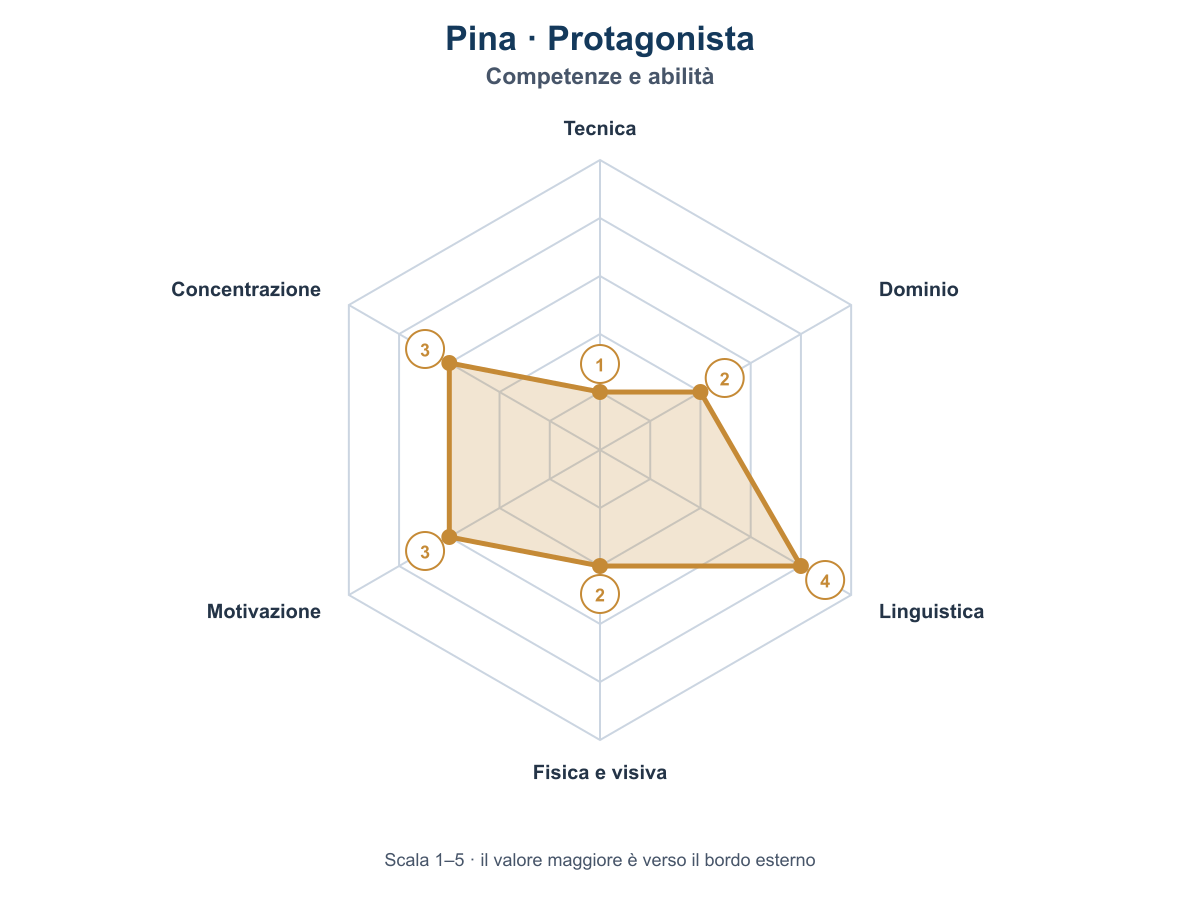
\includegraphics[width=0.88\linewidth]{assets/phase-b-persona-pina-skills.png}

\begin{longtable}{@{}p{0.24\linewidth}p{0.10\linewidth}p{0.59\linewidth}@{}}
\toprule
\textbf{Dimensione} & \textbf{1--5} & \textbf{Motivazione del punteggio} \\
\midrule
Tecnica & 1 & Non usa computer e dipende da aiuto per credenziali e flussi nuovi. \\
Dominio & 2 & Conosce visite ricorrenti, ma non canali e regimi amministrativi. \\
Linguistica & 4 & Comprende bene l'italiano comune; il lessico tecnico crea esitazione. \\
Fisica e visiva & 2 & Presbiopia e tremore rendono difficili testi e bersagli piccoli. \\
Motivazione & 3 & Vuole autonomia, ma l'ansia cresce dopo pochi tentativi falliti. \\
Concentrazione & 3 & Procede con cura; interruzioni ed errori riducono la continuità. \\
\bottomrule
\end{longtable}

\fieldheading{Scenario: la visita diabetologica di controllo}

Pina deve prenotare la visita semestrale. Recupera l'impegnativa, controlla
gli impegni sul calendario cartaceo e prova ER Salute. Non ricorda la password
SPID, confonde ``Prenota'' con ``Informazioni'' e non comprende un errore.
Dopo due tentativi chiama Elena durante una riunione. Il compito richiede
circa 10--15 minuti prima della richiesta di aiuto. Il successo consiste nel
comprendere il passo corrente, scegliere sede e data consapevolmente e
ricevere una conferma verificabile senza sostituzione da parte della figlia.
I rischi principali sono errore di selezione, frustrazione, abbandono e
rinuncia futura.

\fieldheading{Implicazioni di design}

\begin{itemize}
\item {[}P-01{]} L'autenticazione deve ridurre il carico di memoria e offrire recupero guidato; per attività solo consultive va evitata un'autenticazione ripetuta non necessaria.
\item {[}P-02{]} Azioni e bersagli devono essere grandi, distinti per forma, testo e icona, non soltanto per colore.
\item {[}P-03{]} Il linguaggio deve essere semplice e rassicurante, con conseguenze e conferme esplicite.
\item {[}U1-01{]} Il percorso per una visita ricorrente deve conservare il contesto e ridurre i passaggi senza decidere al posto dell'utente.
\item {[}U1-02{]} Prima dell'abbandono, un errore deve indicare causa, recupero e modalità di richiesta d'aiuto.
\end{itemize}

\cardsection{Documento 02b: Persona and Use Case card: personaggio secondario}

\personaphoto{Elena Ferretti}

\fieldheading{Identità, ruolo e segmento}

\begin{longtable}{@{}p{0.25\linewidth}p{0.69\linewidth}@{}}
\toprule
Nome e livello & Elena Ferretti --- personaggio secondario, caregiver di Pina \\
Segmento & Segmento B: caregiver familiare sempre reperibile a distanza, intermediaria \\
Profilo & 52 anni, impiegata amministrativa, vive a Bologna; famiglia, lavoro e assistenza alla madre \\
Dispositivi & PC e smartphone usati quotidianamente; elevata familiarità con servizi digitali \\
Vincoli & Poco tempo, interruzioni, carico emotivo e rischio di confondere profili o prenotazioni \\
\bottomrule
\end{longtable}

\begin{quote}
\emph{``Vorrei che mia madre potesse cavarsela da sola per le cose semplici, così mi preoccuperei solo per l'importante.''}

\small Citazione sintetica: ipotesi narrativa da sostituire o corroborare con
evidenze anonime delle interviste.
\end{quote}

\evidencestatus{Profilo provvisorio derivato dal Segmento B e dalle domande
B1--B6. La relazione con Pina esplicita il rapporto HPHP, ma frequenza e peso
dell'assistenza devono essere validati.}

\fieldheading{Comportamenti, esperienza e rete di aiuto}

Elena gestisce prenotazioni e disdette da remoto, spesso durante il lavoro.
Conosce CUPweb ed ER Salute, ma deve ricostruire dati, credenziali e intenzione
della madre a ogni richiesta. Accetta la delega solo se vede chiaramente per
chi sta agendo, che cosa cambierà e se Pina sarà informata. Il suo obiettivo è
ridurre le emergenze senza perdere la possibilità di intervenire nei casi
complessi; teme errori sul profilo sbagliato e notifiche insufficienti.

\fieldheading{Competenze e abilità (C\&A)}

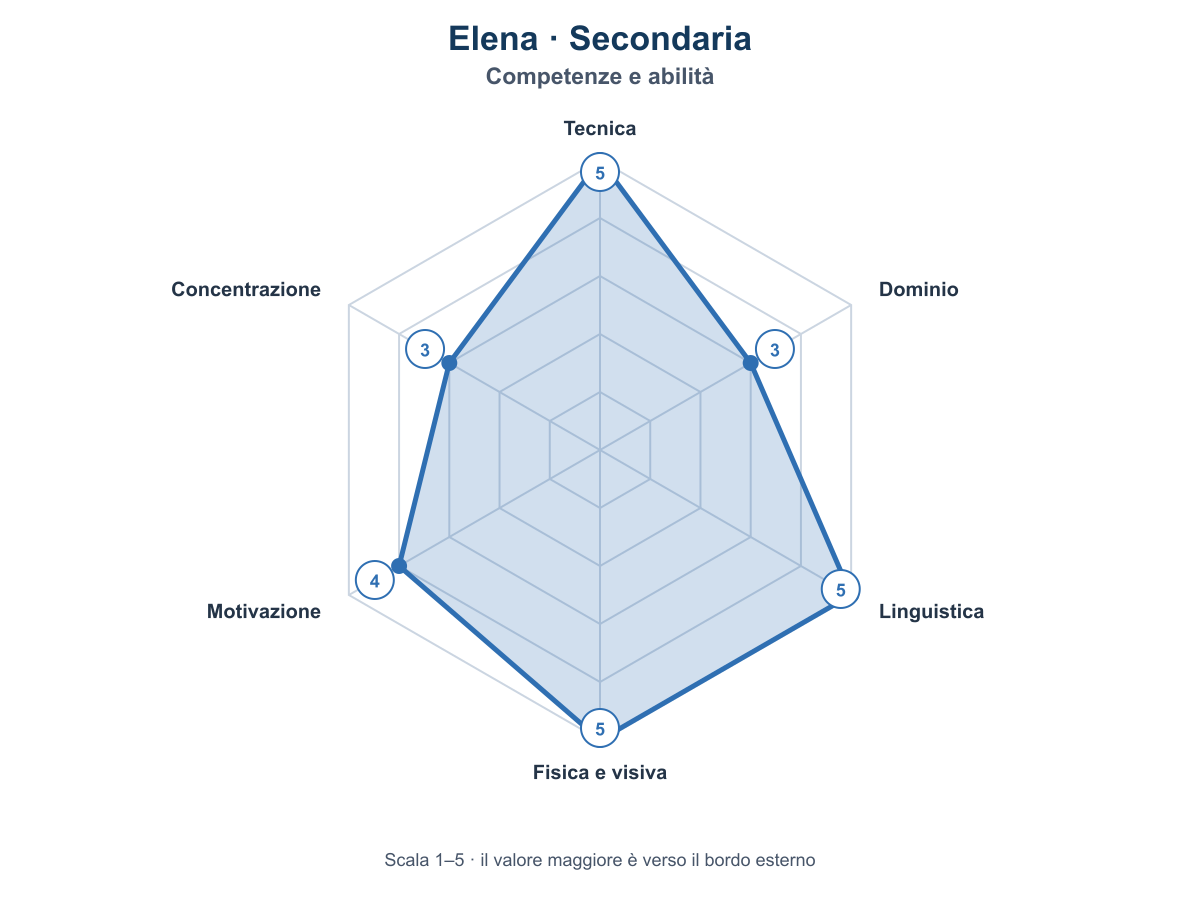
\includegraphics[width=0.88\linewidth]{assets/phase-b-persona-elena-skills.png}

\begin{longtable}{@{}p{0.24\linewidth}p{0.10\linewidth}p{0.59\linewidth}@{}}
\toprule
\textbf{Dimensione} & \textbf{1--5} & \textbf{Motivazione del punteggio} \\
\midrule
Tecnica & 5 & Usa quotidianamente PC, smartphone e servizi autenticati. \\
Dominio & 3 & Ha esperienza pratica, ma deve ricostruire prescrizioni e regimi. \\
Linguistica & 5 & Legge rapidamente anche testi amministrativi. \\
Fisica e visiva & 5 & Non emergono limitazioni rilevanti per il compito. \\
Motivazione & 4 & È motivata a proteggere Pina e a ridurre le interruzioni. \\
Concentrazione & 3 & Le richieste arrivano mentre lavora o gestisce la famiglia. \\
\bottomrule
\end{longtable}

\fieldheading{Scenario: la disdetta urgente dall'ufficio}

Durante il lavoro Elena riceve una chiamata da Pina: una visita va disdetta.
Deve identificare profilo e appuntamento corretti, controllare le conseguenze,
completare l'azione e rassicurare la madre in circa 5 minuti, prima di una
riunione. Il successo consiste in una disdetta verificabile, senza errore di
persona o appuntamento, con stato visibile a entrambe. Il rischio è che la
velocità spinga Elena a sostituirsi stabilmente a Pina.

\fieldheading{Implicazioni di design}

\begin{itemize}
\item {[}P-04{]} Il caregiver deve avere una visibilità chiara e proporzionata sulle prenotazioni autorizzate del familiare, con identità sempre evidente.
\item {[}P-05{]} La delega deve essere progressiva: Pina conserva le azioni semplici, Elena interviene nei casi complessi senza sorveglianza continua.
\item {[}U2-01{]} La disdetta deve richiedere pochi passaggi, distinguere appuntamenti simili e rendere esplicite le conseguenze.
\item {[}U2-02{]} Lo stato aggiornato e notifiche concordate devono ridurre telefonate di verifica e interventi d'emergenza.
\end{itemize}

\cardsection{Documento 02c: Persona and Use Case card: personaggio aggiuntivo}

\personaphoto{Renato Bellini}

\fieldheading{Identità, ruolo e segmento}

\begin{longtable}{@{}p{0.25\linewidth}p{0.69\linewidth}@{}}
\toprule
Nome e livello & Renato Bellini --- personaggio aggiuntivo di livello inferiore \\
Segmento & Segmento A: ``nuovo utente digitale'' 65--74, utente diretto moderatamente autonomo \\
Profilo & 70 anni, pensionato (ex assistente di biblioteca), vive a Forlì con la moglie; figlio adulto nelle vicinanze \\
Dispositivi & Tablet e smartphone; messaggistica, e-mail e SPID usato occasionalmente \\
Vincoli & Affaticamento visivo, rigidità delle mani, esitazione davanti a terminologia sanitaria o amministrativa ambigua \\
\bottomrule
\end{longtable}

\begin{quote}
\emph{``Se capisco cosa sto confermando, preferisco fare da solo e chiedere aiuto solo quando serve.''}

\small Citazione sintetica: ipotesi narrativa da sostituire o corroborare con
evidenze anonime delle interviste.
\end{quote}

\evidencestatus{Persona provvisoria costruita dal Segmento A e dalle domande
A1--A6. Serve come controllo del progetto, non come risultato già validato:
biografia, comportamenti, scenario e punteggi potranno cambiare dopo le
interviste.}

\fieldheading{Comportamenti, esperienza e rete di aiuto}

Renato prenota in autonomia quando riconosce il tipo di prestazione e il
regime; in alternativa telefona o chiede al figlio di verificare, non di
operare al suo posto. Ha già usato SPID e provato CUPweb/ER Salute, ma si
ferma davanti a etichette come ``SSN'', ``libera professione'' o costi non
immediatamente visibili. Teme una conferma onerosa o nella sede sbagliata.
Si sente autonomo se può leggere con calma, tornare indietro senza perdere le
scelte e verificare un riepilogo prima dell'invio. Descrive il proprio rapporto
con il digitale come positivo, purché il servizio non lo tratti da inesperto.

\fieldheading{Competenze e abilità (C\&A)}

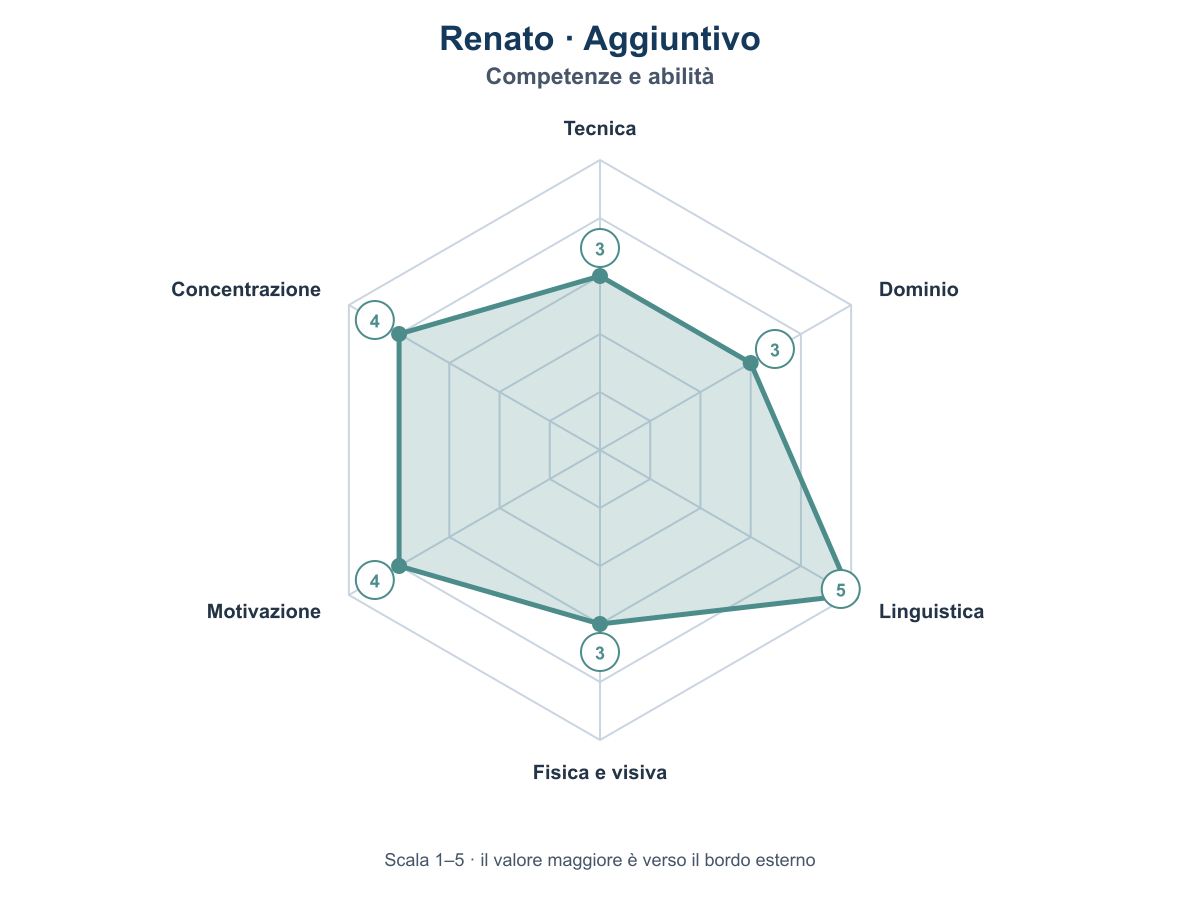
\includegraphics[width=0.88\linewidth]{assets/phase-b-persona-renato-skills.png}

\begin{longtable}{@{}p{0.24\linewidth}p{0.10\linewidth}p{0.59\linewidth}@{}}
\toprule
\textbf{Dimensione} & \textbf{1--5} & \textbf{Motivazione del punteggio} \\
\midrule
Tecnica & 3 & Usa servizi comuni e SPID, ma non automatizza procedure nuove. \\
Dominio & 3 & Conosce il percorso sanitario, non sempre regimi e conseguenze. \\
Linguistica & 5 & Legge e comprende bene; l'ambiguità terminologica è il limite. \\
Fisica e visiva & 3 & Affaticamento e rigidità richiedono buona leggibilità e bersagli ampi. \\
Motivazione & 4 & Preferisce operare da solo e considera l'aiuto una verifica mirata. \\
Concentrazione & 4 & Riesce a seguire il flusso se può fermarsi e riprendere senza perdere dati. \\
\bottomrule
\end{longtable}

\fieldheading{Scenario: il controllo oculistico senza chiamare il figlio}

Renato riceve l'impegnativa e prova a prenotare dal tablet. Confronta due
sedi, consulta il calendario e si ferma quando non distingue con certezza
SSN e libera professione. Vorrebbe verificare il significato senza perdere le
scelte già fatte. Stima di concludere in 8--10 minuti. Il successo consiste
nel prenotare sede, data e regime voluti, comprendere il costo e conservare
una conferma; chiedere una spiegazione non deve obbligarlo a cedere il compito
al figlio. I rischi sono affaticamento, scelta costosa e percezione di un
servizio paternalistico.

\fieldheading{Implicazioni di design}

\begin{itemize}
\item {[}P-06{]} Le spiegazioni devono essere progressive e facoltative: disponibili nel punto di dubbio, senza rallentare chi ha già compreso.
\item {[}P-07{]} Testo, spaziatura e bersagli devono restare leggibili e azionabili anche con affaticamento visivo e precisione ridotta.
\item {[}P-08{]} Regime, costo e conseguenze devono essere visibili in linguaggio rispettoso, senza semplificazioni paternalistiche.
\item {[}U3-01{]} Consultare una spiegazione, tornare indietro o chiedere aiuto non deve cancellare le scelte già effettuate.
\item {[}U3-02{]} Prima della conferma, un riepilogo deve mostrare prestazione, sede, data, regime e costo.
\end{itemize}

\cardsection{Documento 03: Cast card}

\fieldheading{Gerarchia, relazione e funzione nel cast}

\begin{enumerate}
\item \textbf{Pina --- protagonista.} Caso guida per accessibilità, fiducia e autonomia minima.
\item \textbf{Elena --- secondaria.} Caregiver a distanza collegata a Pina; rende visibile il conflitto tra assistenza e sostituzione.
\item \textbf{Renato --- aggiuntivo.} Controlla che le soluzioni per Pina non penalizzino efficienza, dignità e autonomia di un anziano più competente.
\end{enumerate}

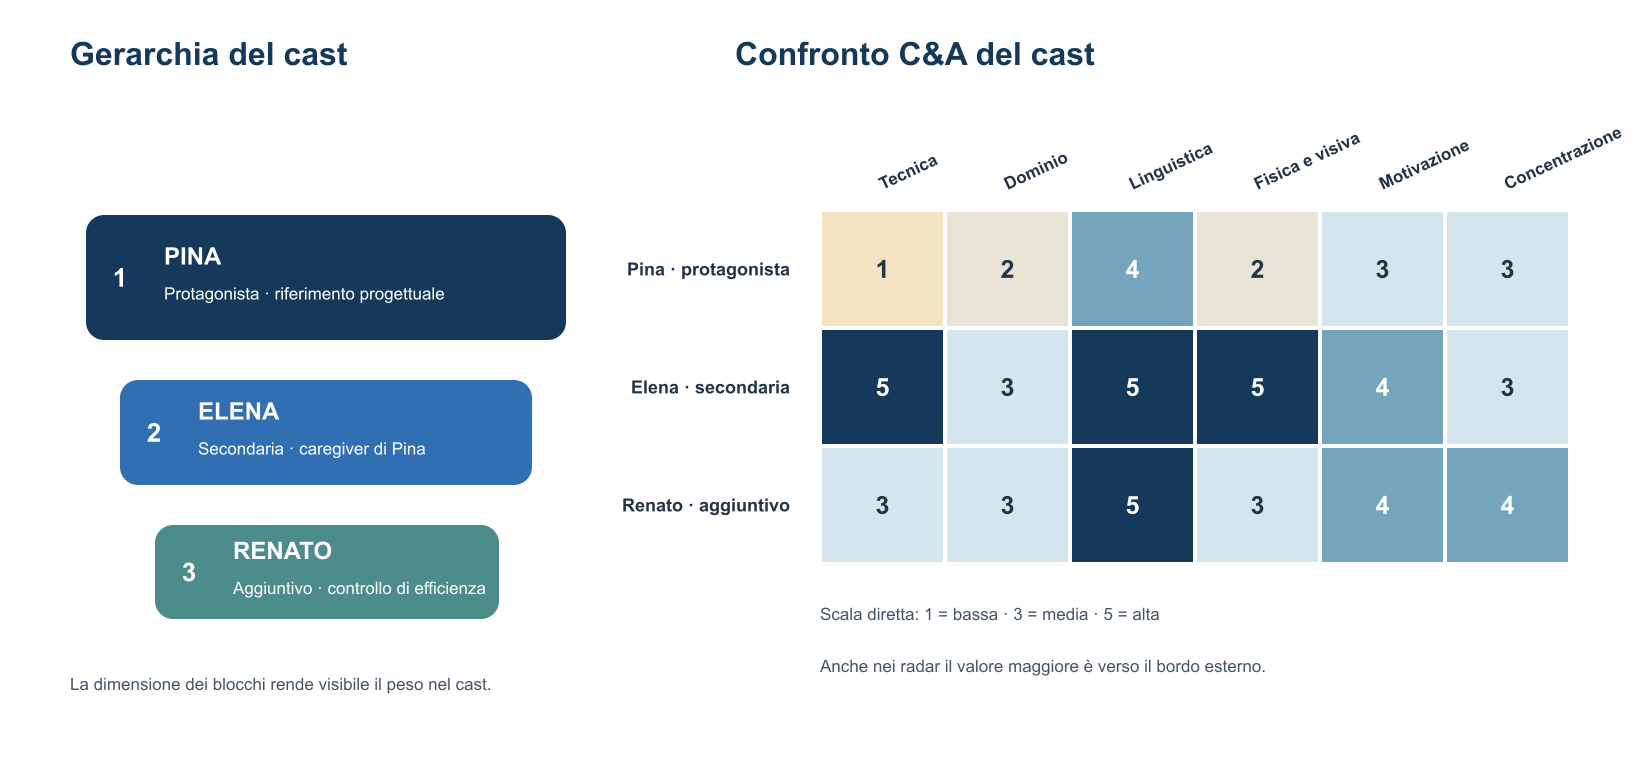
\includegraphics[width=\linewidth]{assets/phase-b-personas-comparison.png}

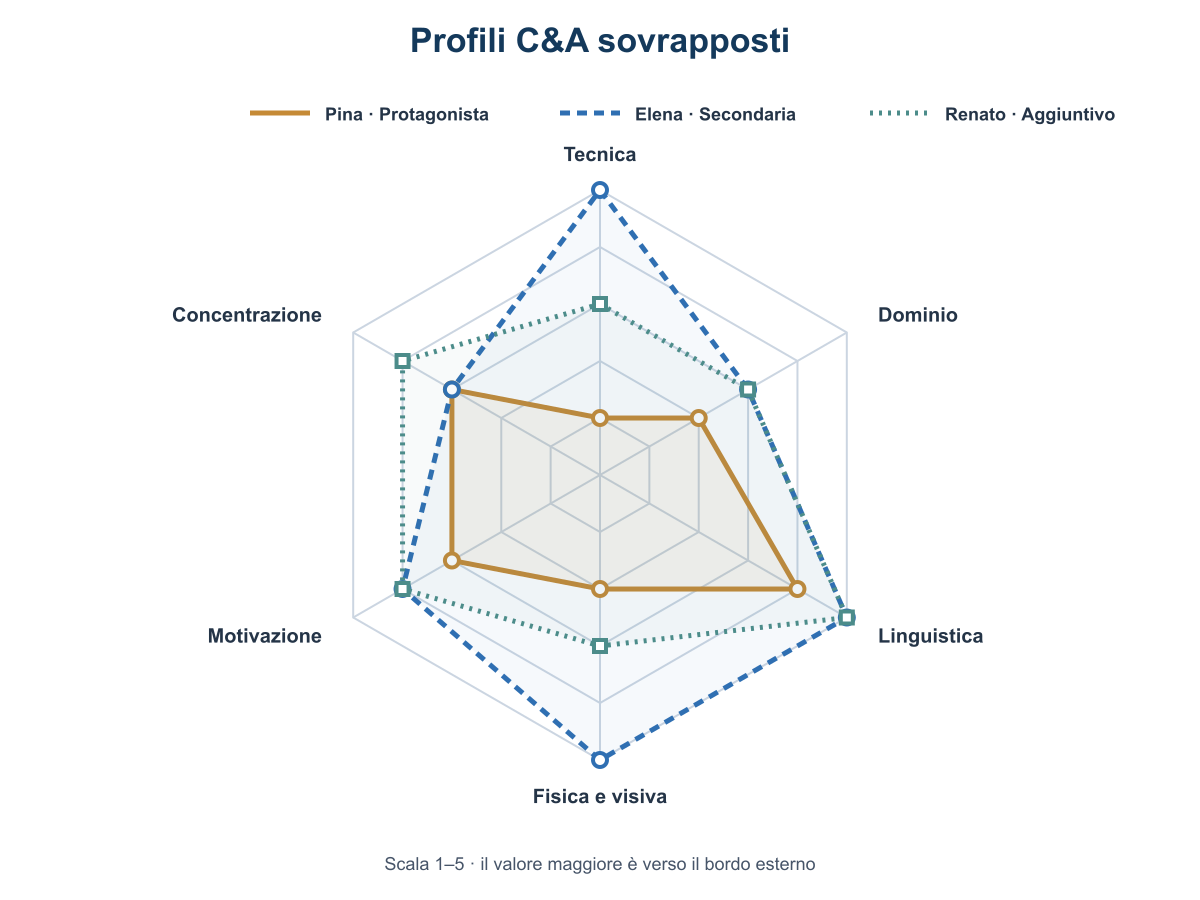
\includegraphics[width=0.90\linewidth]{assets/phase-b-personas-overlay.png}

Il workbook \texttt{phase-b-personas-and-cast.xlsx} contiene valori sorgente,
motivazioni, grafici radar editabili, matrice comparativa e schede scenario.
La heatmap e tutti i radar usano la scala diretta 1--5: il valore 1 è vicino
al centro, mentre il valore 5 raggiunge il bordo esterno. Il radar sovrapposto
permette di confrontare il profilo complessivo delle tre persone.

\fieldheading{Motivazione della selezione e alternative scartate}

Pina ed Elena coprono i due segmenti prioritari e la relazione HPHP centrale.
Renato introduce una variazione interna al Segmento A e verifica il bilanciamento
tra semplicità ed efficienza. Sono state rinviate: una caregiver convivente con
competenza media, perché aggiunge poca variabilità rispetto a Elena; una figura
sanitaria o di farmacia, perché esterna ai segmenti intervistati; una persona
completamente dipendente, perché sarebbe un caso limite artificiale senza
evidenze sufficienti. Anche gli scenari di sola consultazione e di modifica
anagrafica sono rinviati perché meno rappresentativi del problema di
prenotazione e assistenza emerso in Fase A.

\fieldheading{Matrice persona -- domande di Fase A -- validazione}

\begin{longtable}{@{}p{0.15\linewidth}p{0.31\linewidth}p{0.28\linewidth}p{0.18\linewidth}@{}}
\toprule
\textbf{Persona} & \textbf{Elemento} & \textbf{Domanda/evidenza Fase A} & \textbf{Stato} \\
\midrule
Pina & Prenotazione attuale, tentativi digitali, aiuto, paure e autonomia & Segmento A, domande A1--A6 & Ipotesi da validare \\
Pina & Vincoli visivi e motori; punteggi C\&A & Domande A4--A6; osservazione futura & Ipotesi da validare \\
Elena & Carico, urgenza e gestione da remoto & Segmento B, domande B1--B2 e B6 & Ipotesi da validare \\
Elena & Delega, fiducia, visibilità e controllo & Domande B3--B5 & Ipotesi da validare \\
Renato & Canali attuali e tentativi CUPweb/ER Salute & Domande A1--A2 & Ipotesi da validare \\
Renato & Quando chiede aiuto e che cosa teme & Domande A3--A4 & Ipotesi da validare \\
Renato & Condizioni di autonomia e rapporto con il digitale & Domande A5--A6 & Ipotesi da validare \\
\bottomrule
\end{longtable}

\fieldheading{Conflitti progettuali}

\begin{itemize}
\item Una guida sempre visibile sostiene Pina ma può rallentare Renato: servono spiegazioni progressive e richiudibili.
\item Le scorciatoie utili a Elena non devono nascondere identità, stato o conseguenze dell'azione.
\item La supervisione rassicura il caregiver, ma può diventare sorveglianza o sostituzione dell'utente diretto.
\item Controlli grandi e spaziati devono convivere con una densità informativa sufficiente per chi opera rapidamente.
\end{itemize}

\fieldheading{Requisiti cumulativi del cast}

\begin{itemize}
\item {[}C-01{]} (= P-01+P-02+P-03) Il servizio deve essere utilizzabile con competenza tecnica minima, azioni visibili e tono rassicurante.
\item {[}C-02{]} (= P-04+P-05) Visibilità e delega devono sostenere una supervisione leggera, autorizzata e non sostitutiva.
\item {[}C-03{]} (= U1-01+U2-01) Prenotazione ricorrente e disdetta devono ridurre passaggi e ambiguità mantenendo il controllo dell'utente.
\item {[}C-04{]} (= U1-02+U2-02) Errori e cambi di stato devono offrire recupero comprensibile e notifiche concordate.
\item {[}C-05{]} (= P-03+P-04) Identità, oggetto e conseguenze dell'azione devono essere espliciti per utente diretto e caregiver.
\item {[}C-06{]} (= P-06+P-08) Spiegazioni progressive devono chiarire termini, regime, costo e conseguenze senza infantilizzare.
\item {[}C-07{]} (= P-02+P-07) Gerarchia, leggibilità, spaziatura e dimensione dei bersagli devono supportare vincoli visivi e motori.
\item {[}C-08{]} (= U3-01+U3-02) Il sistema deve conservare le scelte durante consultazione e aiuto, quindi mostrare un riepilogo completo prima della conferma.
\end{itemize}
